\section{Rendu : Stratégie et conception}

\subsection{Stratégie de rendu d'un état}

Afin de pouvoir réaliser un rendu imagé de notre jeu RISK, il nous faut tout d’abord réaliser un rendu des différents éléments qui composent notre jeu. Grâce aux outils de la librairie SFML, l'affichage se fera dans une fenêtre avec laquelle le joueur pourra intéragir. 

Comme pour la mise en place des différents états, nous allons différencier le rendu des éléments fixes (à savoir la map du jeu avec les pays et les continents) et le rendu des éléments mobiles amenés à se déplacer pendant le jeu (à savoir les armées et les cartes). 

Pour cela, le choix s'oriente vers une stratégie assez bas niveau et relativement proche du fonctionnement des unités graphiques. Plus précisément, le découpage se fait en différents plans nommés layers. Naturellement, un plan concernera les éléments statiques et affichera donc la carte, un autre sera consacré aux armées et un dernier s'occupera des cartes.

Pour la carte, le monde et la division des différents pays a été réalisé au préalable sur Tiled. Nous pouvons donc charger le fichier image comme texture et utiliser un sprite pour l'afficher dans la fenêtre du jeu. Nous pourrons ainsi redimensionner la carte principale comme nous le souhaitons.
Pour les éléments mobiles, nous utiliserons là encore des textures trouvées sur internet pour mettre en place nos armées et les cartes. L'utilisation des sprites permettra de faire varier les couleurs par exemple. 

Avant de commencer à afficher les éléments mobiles, nous avons déterminé dans quelle zone de la fenêtre chaque pays se trouvait. Puis, nous déterminons approximativement le centre de cette zone afin d'y placer les pions correspondant aux armées par la suite. Cela permettra également de savoir dans quel pays un joueur clique avec la souris. 


\subsection{Conception logiciel}

Le diagramme des classes pour les rendus est présenté sur la figure \ref{fig:render}.
\newline

\textbf{Affichage:} Le diagramme render se veut finalement assez simple. Nous l'avons beaucoup modifié afin de ne garder que les éléments et méthodes dont nous avions besoin. 
D'autres méthodes s'y ajouteront pour ajouter un menu où plusieurs actions et informations seront disponibles. Cela permettra de ne plus passer par le terminal ce qui n'est pas encore le cas pour le moment. 
\newline 

La méthode \textbf{AfficheMap} permet tout simplement d'afficher la carte du monde permettant de joueur. La fenêtre est lancée dans le main.cpp qui appelle en premier lieu cette méthode afin d'initialiser le plateau du jeu. 
\newline 

La méthode \textbf{AfficheArmées} initialise un pion "armée" dans chacun des territoires. Ce pion a pour le moment une couleur grise correspondante à l'état de l'initialisation. Par la suite, il prendra la couleur du joueur auquel le pays appartient.  
\newline 

La méthode \textbf{AfficheNombre} affichera à côté du pion "armée", le nombre d'armées présentes sur ce territoire. Cela permettra au joueur de décider avec combien d'armée, il souhaite attaquer un territoire ennemi. 
\newline

La méthode \textbf{PaysClic} permet de déterminer les clics réalisés sur la fenêtre. Ainsi, dans un second temps, le choix des pays attaquants, et du nombre d'armées se fera directement dans la fenêtre du jeu. Dans un premier temps, cela se fera dans le terminal. 




\begin{landscape}
    \begin{figure}[!htbp]
        \centering
        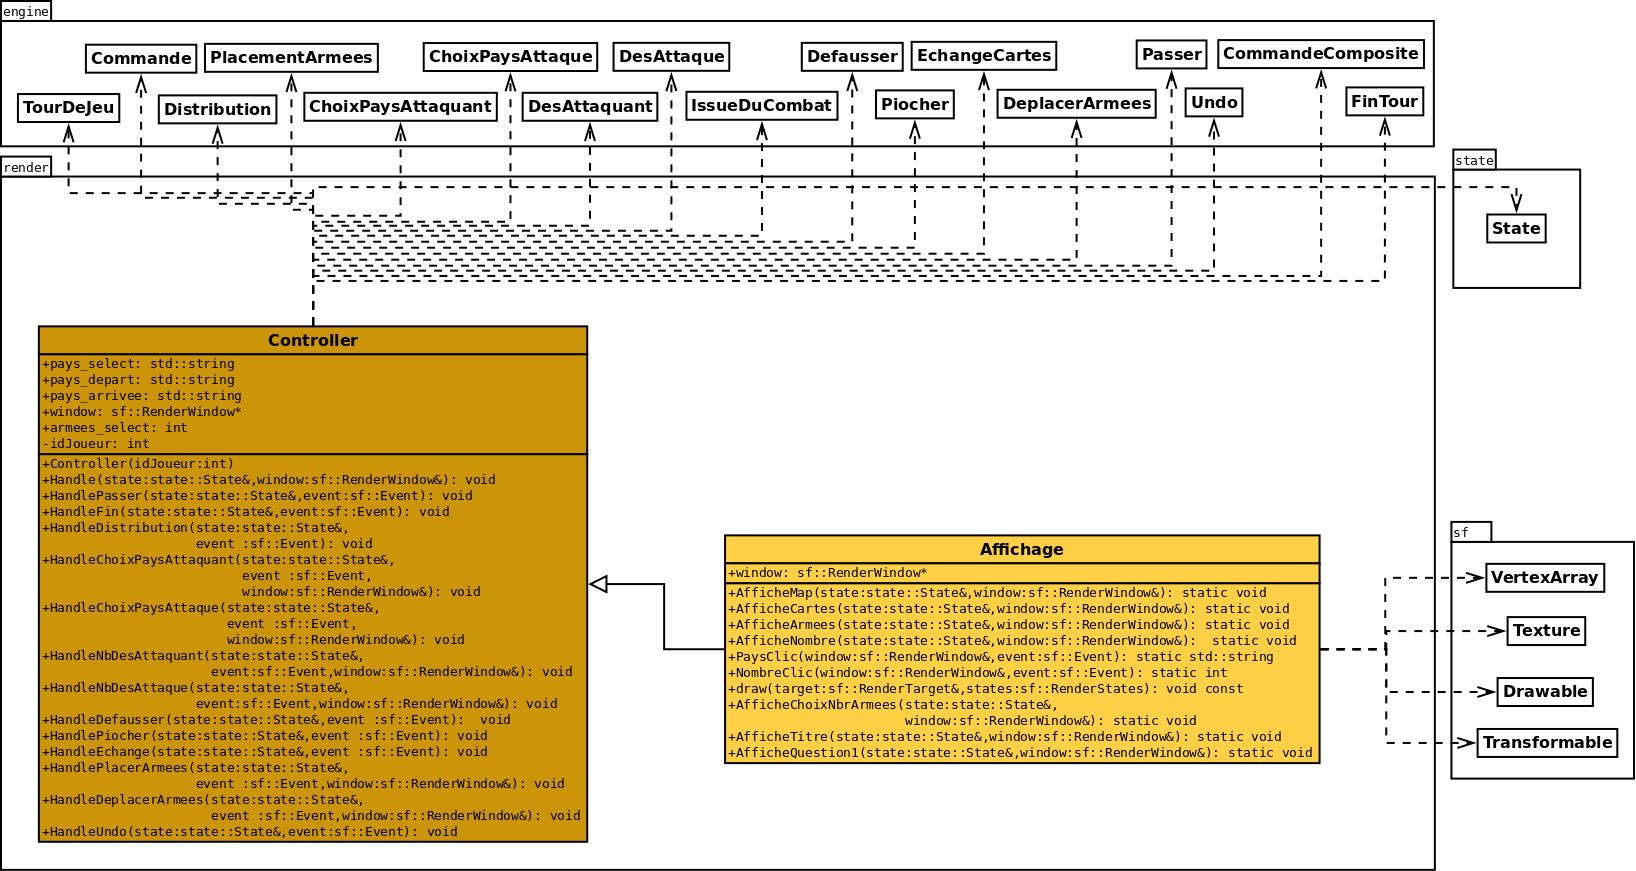
\includegraphics[width=21cm]{Images/render.png}
        \caption{Diagramme des rendus}
        \label{fig:render}
    \end{figure}
\end{landscape}